\chapter{Cronograma y Costos}
% \section{State of the Art}

\section{Cronograma}

Para el desarrollo de las actividades relacionadas con los objetivos, se estima un tiempo de trabajo de doce meses separando las actividades en cuatro grandes fases:

\begin{itemize}
    \item Estudio de alineadores forzados 
    \item Recolección de recursos anotados
    \item Diseño e implementación 
    \item Anotación de corpus existentes
\end{itemize}

Se inicia con un mes dedicado al análisis del arte, contemplando el análisis de los alineadores abiertos existentes, los corpus abiertos anotados y los corpus abiertos no anotados.

Finalizado el estado del arte, se dedican tres meses para el estudio de los alineadores automáticos abiertos, separando un mes para la adecuación de ambientes y puesta en marcha de los alineadores abiertos existentes, entendiendo las técnicas y tecnologías relacionados con cada uno, buscando seleccionar la mejor aproximación para la implementación propia y los últimos dos meses para el análisis teórico de los propuestas de alineadores forzados. Con estas actividades se cierra la primera fase de estudio de los alineadores forzados, teniendo en este punto un análisis comparativo de las herramientas existentes, así también como una visión nocional de los corpus anotados y no anotados abiertos.

La fase dos toma dos meses para el análisis en profundidad de los corpus abiertos anotados y no anotados para el lenguaje español, entendiendo en cada uno sus características de duración y locutores, el nivel de anotación en caso de los anotados y características prosódicas que pueden ser relevantes para la anotación automática posterior. Al final de esta etapa se tendrá un documento descriptivo a profundidad de los recursos abiertos anotados y no anotados para el lenguaje español.

En la fase tres se dedicarán tres meses para la implementación del alineador forzado, teniendo como base de pruebas corpus anotados a un nivel fino, siendo lo ideal una anotación a nivel fonético. Se realizará el desarrollo de forma iterativa iniciando con corpus sin ruido y mejorando la robustez del alineador en ambientes ruidosos. Al final de esta etapa existirá un nuevo alineador forzado de código abierto que minimiza la diferencia entre los intervalos de anotación detectados con respecto a los especificados en los corpus anotados seleccionados.

La última fase usa el alineador previamente implementado y realiza una anotación en un corpus abierto de larga duración en el lenguaje español. Se realizarán los ajustes necesarios para una buena anotación de este corpus y se liberará la anotación para ser usada en posteriores investigaciones.

Se muestra un diagrama de Gantt con los estimados de tiempos para cada actividad en la figura \ref{img:schedule}

\begin{landscape}
\begin{figure}[H]

\centering
\caption{Cronograma}
\label{img:schedule}
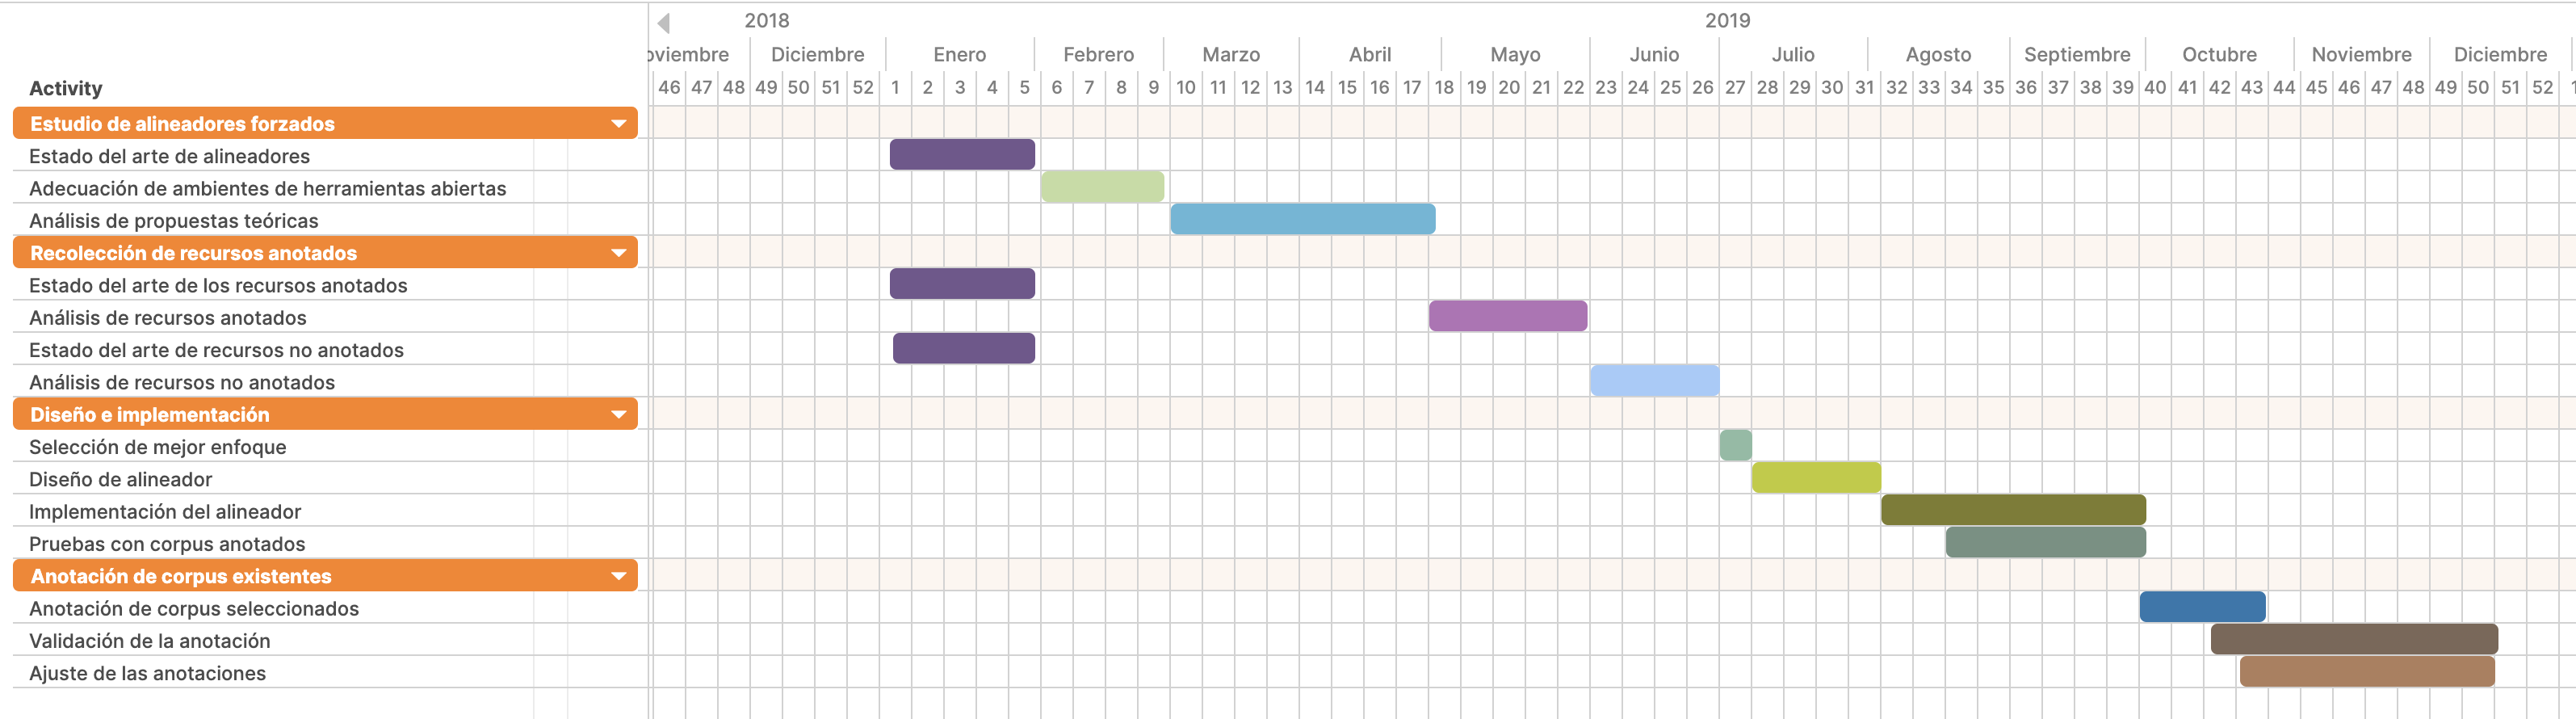
\includegraphics[scale=0.40]{images/schedule.png}

\end{figure}
\end{landscape}


\section{Costos}
% \section{Costos}

Para el desarrollo del proyecto, cuya duración se estima de 12 meses, se plantea una estructura de costos considerando el costo de hora del investigador principal, su asesor de tesis y horas hombre de validación manual de la anotación automática como proceso de verificación del corpus anotado automáticamente como costos de recurso humano. También se consideran costos de infraestructura, que contemplan una estación de cómputo para el investigador principal así como recursos en nubes públicas para el alojamiento de aplicaciones web relacionadas con el proyecto. También se espera que como resultado del proyecto se publique un artículo en una revista indexada y se participe en un congreso internacional, para lo cual se estiman los costos de viáticos y honorarios de la casa publicadora. También se estima un presupuesto relacionado con materiales bibliográficos pagos que deban adquirirse en el proceso del proyecto. 

Se detallan los costos estimados en el cuadro \ref{tab:cost_structure}



\begin{table}[]
\centering
\caption{Presupuesto}
% \caption{Speech English Corpus}
\label{tab:cost_structure}
\begin{tabular}{|l|l|l|l|}
\toprule
Cantidad                                   & Cantidad       & Valor Unitario   & Total          \\
\hline
Horas de investigación                     & 1056           & 25000   & 26400000 \\
\hline
Horas director de tesis                    & 52             & 100000  & 5200000  \\
\hline
Horas validación manual                    & 240            & 5600    & 1344000  \\
\hline
Equipo de cómputo                          & 1              & 7500000 & 7500000  \\
\hline
Alojamiento mensual de recursos en la nube & 12             & 100000  & 1200000  \\
\hline
Publicaciones                              & 1              & 1800000 & 1800000  \\
\hline
Conferencias                               & 1              & 4000000 & 4000000  \\
\hline
Material Bibliográfico                     & 1              & 2000000 & 2000000  \\
\hline
Total                                      &                &         & 49444000 \\
\hline
\end{tabular}
\end{table}